% PWr general use template version 04.11.2018
%----------------------------------------------------------------------------------------
%	PACKAGES AND DOCUMENT CONFIGURATIONS
%----------------------------------------------------------------------------------------
\documentclass{article}
\usepackage{siunitx} % Provides the \SI{}{} and \si{} command for typesetting SI units
\usepackage{graphicx} % Required for the inclusion of images
%\usepackage{natbib} % Required to change bibliography style to APA
\usepackage{amsmath} % Required for some math elements
\usepackage{float}
\graphicspath{ {../../results/} }
\setlength\parindent{12pt} % Removes all indentation from paragraphs
%\usepackage{times} % Uncomment to use the Times New Roman font
\usepackage[export]{adjustbox}

% Polish language
\usepackage[utf8]{inputenc}
\usepackage{polski}
\usepackage[polish]{babel}

\usepackage[top=1in, bottom=1.25in, left=1.25in, right=1.25in]{geometry} % Margin
\usepackage{listings} % Code
\usepackage{indentfirst} % \par Paragraphs
\usepackage{multicol} % Multicolumn itemize
\usepackage{color} % Colored text
\usepackage[square,sort,comma,numbers]{natbib}

\usepackage{amsmath}
\usepackage[ruled,longend]{algorithm2e}
\renewcommand*{\listalgorithmcfname}{Spis algorytmów}
\renewcommand*{\algorithmcfname}{Algorytm}
%\renewcommand*{\algorithmautorefname}{heuristic}
%\renewcommand{\labelenumi}{\alph{enumi}.} % Numbers in enumerate changed to a, b, c, ...

%\lstdefinestyle{sharpc}{language=[Sharp]C, frame=lr, rulecolor=\color{blue!80!black}}
%\lstdefinestyle{cpp}{language=C++, frame=lr}

%----------------------------------------------------------------------------------------
%	DOCUMENT INFORMATION
%----------------------------------------------------------------------------------------

\title{Analiza i ocena bezpieczeństwa systemów usługowych i IoT \\ Ocena skuteczności różnych metod łamania haseł \\ \textsc{Raport 2}}
\author{Jan \textsc{Pajdak} \\ Wojciech \textsc{Słowiński} \\ Maria \textsc{Filemonowicz}}
\date{\today}

\begin{document}
	\bibliographystyle{plainnat}
	%\lstset{style=cpp}
	\maketitle
	\begin{center}
		\begin{tabular}{l r}
			Prowadzący: &  Dr hab. inż. Grzegorz \textsc{Kołaczek}
		\end{tabular}
	\end{center}
	
	\newpage
	\tableofcontents
	
	%----------------------------------------------------------------------------------------
	%	SECTION 0
	%----------------------------------------------------------------------------------------
	
	%\begin{multicols}{2}
	%	\begin{itemize}
	%		\item
	%	\end{itemize}
	%\end{multicols}
	
	%\newpage
	%\section{Title}}
	%\subsection{Title}
	%\par Text
	
	%\begin{itemize}
	%	\item\textit{Text} - Desc
	%\end{itemize}
	
	%\begin{enumerate}
	%	\item Desc
	%\end{enumerate}
	
	%\begin{center}
	%	\includegraphics[scale=0.6, center]{images\}
	%\end{center}
	
	%\begin{lstlisting}[basicstyle=\small]
	%	programming code
	%\end{lstlisting}
	
	%----------------------------------------------------------------------------------------
	%	SECTION 1
	%----------------------------------------------------------------------------------------
	\newpage
	\section{Cel eksperymentu}
	Hasła tekstowe to obecnie najpopularniejsza metoda uwierzytelniana używana do ograniczania dostępu do zasobów takich jak serwisy internetowe czy konta pocztowe przez osoby nieupoważnione. Zabezpieczenia tego typu są łatwe w użyciu jednakże proste do złamania — w ramach eksperymentu analizowane będzie łamanie haseł przy użyciu algorytmów \textit{BFM} oraz \textit{Weira}.
	
	Eksperyment będzie przeprowadzony przy użyciu bazy realnych haseł, które następnie będą badane pod kątem odporności na złamanie przez poszczególne algorytmy.
	
	%----------------------------------------------------------------------------------------
	%	SECTION 2
	%----------------------------------------------------------------------------------------
	\section{Plan eksperymentu}
	\subsection{Źródło danych}
	Jako źródło danych wybrana została baza danych znaleziona w roku 2017 przez firmę z branży cyberbezpieczeństwa - \textit{4iQ} \cite{breach}. Baza jest kompilacją informacji z 252 wycieków; zawiera loginy i hasła do ponad 1.4 miliarda kont. Całkowity rozmiar danych to 41.1 GB. Osoba odpowiedzialna za stworzenie bazy danych jest nieznana; dane zostały odkryte przez \textit{4iQ} w \textit{dark web} i można je obecnie pobrać przy użyciu sieci \textit{torrent}.
	
	Dane muszą zostać sformatowane przed użyciem ich w eksperymencie — są one porozdzielane na wiele plików oraz zawierają loginy i adresy poczty elektronicznej powiązane z kontami; te dodatkowe informacje są zbędne. Ze względu na ilość danych badany będzie podzbiór haseł.
	
	\subsection{Planowany przebieg eksperymentu}
	Algorytmy rozważane w niniejszym eksperymencie posiadają wysoką złożoność obliczeniową i czasową, przez co testowanie ich implementacji na dużych zbiorach haseł byłoby bardzo ograniczone przez moc obliczeniową dzisiejszych komputerów i czas potrzebny na przeprowadzenie takich badań. Aby umożliwić przeprowadzenie eksperymentu na o wiele większej bazie haseł, wykorzystane zostaną metody pozwalające na wyliczenie liczby prób potrzebnych do odgadnięcia hasła w obu algorytmach, nazywane \textit{kalkulatorami} \cite{calc}, dzięki którym wyznaczyć można siłę hasła.
	
	\subsection{Technologie}
	Do formatowania bazy haseł wykorzystany został \textit{Python}.
	
	Algorytmy oceniające skuteczność łamania haseł w poszczególnych algorytmach zostały zaimplementowane przy użyciu \textit{Scala}.

	
	\subsection{Metoda oceny}
	\subsubsection{BFM}
	Kalkulator oceny skuteczności algorytmu \textit{BFM} działa następująco:
	\begin{enumerate}
		\item Na podstawie treningowego zbioru haseł określane są:
		\subitem Zbiór pojedynczych znaków alfabetu wraz z częstotliwością ich występowania jako pierwsza litera hasła 
		\subitem Zbiór wszystkich możliwych digramów ułożonych ze znaków w alfabecie wraz z częstotliwością ich występowania, tworzony w następujący sposób:
		\subsubitem Zakładając zbiór treningowy złożony ze znaków \textit{A, B, C}; Jeżeli znak \text{A} ma największe prawdopodobieństwo wystąpienia jako pierwszy, znak \textit{B} ma największe prawdopodobieństwo wystąpienia po \textit{A} a znak \textit{C} ma największe prawdopodobieństwo wystąpienia po \textit{B}, pierwszą próbą odgadnięcia hasła będzie \textit{ABC}.
		\item Na podstawie powstałych zbiorów określona zostaje kolejność zgadywania kolejnych znaków w haśle	
		%\item Dla właściwego zbioru haseł wyznaczana jest liczba wymaganych prób potrzebnych do jego odgadnięcia według następującego wzoru: $ (k-i)N^{L-i} $
		
		\item Dla właściwego zbioru haseł wyznaczana jest liczba wymaganych prób potrzebnych do jego odgadnięcia:
		\subitem \textit{N - długość zbioru znaków w alfabecie}
		\subitem \textit{L - długość zgadywanego hasła}
		\subitem \textit{M - minimalna długość hasła}
		\subitem \textit{CF - liczbę znaków sprawdzanych przed odgadnięciem właściwego pierwszego znaku hasła}
		\subitem \textit{DF(i) - liczba digramów sprawdzanych przed odgadnięciem właściwego i-tego znaku hasła}
		\subitem \textit{i - pozycja znaku w haśle}
		\subitem \textit{k - k-ta próba odgadnięcia hasła}
		\subitem \textit{X - liczba haseł krótszych niż zgadywane}
		\subitem \textit{Y - liczba haseł z niepoprawnie odgadniętą pierwszą literą}
		\subitem \textit{Z - liczba haseł z niepoprawnie zgadniętym i-tym znakiem}
		\subitem \textbf{\textit{Q - liczba prób potrzebnych do odgadnięcia zadanego hasła}}
		
		\subitem $ X = \sum_{l = L}^{l = M} N^l $		
		\subitem $ Y = CF * N^{L-1} $		
		\subitem $ Z = \sum_{i = 2}^{i = L} DF(i) * N^{L - (i + 2)} $		
		\subitem $ Q = X + Y + Z $
		
		\subitem \textit{Jeżeli pierwszy znak nie zostanie odgadnięty poprawnie to wiemy, że algorytm podejmie $ N^{L-1} $ prób, zanim spróbuje odgadnąć hasło z innym znakiem na pierwszej pozycji}
		\subitem \textit{Zgodnie z powyższym, dla k-tej próby odgadnięcia pierwszego znaku wiemy, że algorytm podejmie co najmniej $ (k-1)N^{L-1} $ prób odgadnięcia hasła}
		%\subitem \textbf{\textit{Ostateczna ilość prób odgadnięć to suma prób dla każdego znaku}}
	\end{enumerate}

	\subsubsection{Weir}
	Pojęcia używane w algorytmie Weir'a:
	\begin{itemize}
		\item struktura (\textit{structure}) - opis określający typ każdego znaku w haśle
			\subitem \textit{L} - litera
			\subitem \textit{D} - cyfra
			\subitem \textit{S} - znak specjalny			
		\item (\textit{terminal}) - instancja (hasło) spełniająca założenia struktury
		\item grupa prawdopodobieństwa (\textit{probability group}) - grupa terminali o jednakowym prawdopodobieństwie wystąpienia w zbiorze treningowym
	\end{itemize}
	\textit{Przykład: struktura hasła ''password123!@\#'' to ''LLLLLLLLDDDSSS''} \\ \\
	
	
	Proces tworzenia tablicy z której korzysta algorytm jest bardziej złożony niż w przypadku algorytmu BFM.
	\begin{algorithm}
	$ T \gets \text{nowa tablica}$ \\
	\ForAll{$struktury s$}  
	{
		\ForAll{$grupy\_prawdopodobieństwa pg$}
		{
			\ForAll{$lcs \in pg$}
			{
				$c_{i} = $ liczba wystąpień $lcs$ \\
				$p_{i} = $ prawdopodobieństwo wystąpienia $lcs$ w zbiorze treningowym
			}
			$probability=\prod p_{i}$ \\
			$size=\prod c_{i}$ \\
			$T.add: \quad pg,probability,size$
		}		
	}
	$Sort(T) \text{ by } probability$
	%add to each value in t the sum of prior size values
	\caption{Pseudokod opisujący proces tworzenia tablicy używanej w kalkulatorze Weir'a}
	\end{algorithm}
	% todo: algorithm -> algorytm w nagłówku
	% todo: opisać co to lcs
	% todo: reszta algo
	\subsubsection{Estymator siły haseł Monte Carlo}
	W celu porównania ze sobą różnych algorytmów, służących do łamania haseł, skorzystano również z estymatora Monte Carlo \cite{montecarlo}, który szacuje liczbę prób potrzebnych do zgadnięcia danego hasła. Na podstawie ciągu treningowego wybierana jest próbka o zadanej długości n haseł na podstawie prawdopodobieństwa ich zgadnięcia w każdym z modeli ataków, wśród której estymator oszacowuje ile haseł z próbki zostanie złamane przed złamaniem podanego hasła, ustalając tym samym przybliżoną liczbę prób potrzebną na jego złamanie. Metoda ta nie jest dokładna, a wyniki są przybliżone i często zależą od różnych parametrów (takich jak wielkość próbki, wielkość ciągu treningowego), jednak pozwala na porównanie wielu modeli ataków oraz różnych polityk tworzenia haseł.

	W implementacji Monte Carlo \cite{montecarloimplementation} wyróżnione zostały modele ataków bazujące na n-gramach, będące rozszerzeniem algorytmu BFM o dłuższe ciągi znaków, oraz model PCFG, który zaproponowany został przez Weira.

	%----------------------------------------------------------------------------------------
	%	SECTION 3
	%----------------------------------------------------------------------------------------
	\newpage
	\section{Przebieg eksperymentu}
	\subsection{Przygotowanie danych}
	Dane znajdujące się w pobranej bazie są podzielone na 1 981 plików, w 54 folderach. Informacje w plikach są przechowywane w formacie \textit{nazwa\_użytkownika:hasło}. Rozmiar plików nie jest stały. Przed przystąpieniem do eksperymentu za pomocą skryptu napisanego w języku \textit{Python} dane zostały uporządkowane tak, by utworzyć łatwy do analizy zbiór haseł. Algorytm wykonuje następujące operacje dla każdego pliku wchodzącego w skład pobranej bazy:
	\begin{enumerate}
		\item Wczytuje pojedynczą linię z pliku
		\item Usuwa część linii zawierającą hasło
		\item Przechodzi do następnej linii jeżeli hasło zawiera znaki inne niż:
			\subitem cyfry
			\subitem litery z alfabetu łacińskiego
			\subitem znaki specjalne	
	\end{enumerate}	
	Tak przygotowana linia jest następnie przydzielana do kategorii i zapisana do odpowiedniego pliku. W eksperymencie rozróżniamy trzy kategorie haseł:
	\begin{enumerate}
		\item \textit{raw} - każde hasło które nie zostało odrzucone po analizie znaków
		\item \textit{regular8} - hasło o długości min. 8 znaków
		\item \textit{comprehensive8} - hasło o długości min. 8 znaków oraz zawierające co najmniej 1 dużą literę, 1 cyfrę i 1 znak specjalny
	\end{enumerate}
	Wymogi kategorii \textit{regular8} oraz \textit{comprehensive8} bazują na popularnych wymogach dotyczących haseł stosowanych w różnych serwisach internetowych. 
	
	Zaledwie \textit{0,5\%} haseł wchodzących w skład bazy spełnia wymogi \textit{comprehensive8}.
	
	%Wielkość plików zawierających dane testowe została ustalona na 500 000 haseł.
	
	\subsubsection{Ciąg treningowy i ciąg walidacyjny}
	Ciąg treningowy to ważna część danych wejściowych, od których zależy skuteczność algorytmów. Dla każdej kategorii haseł został utworzony zbiór składający się z losowo wybranych haseł z odpowiadającej kategorii. Podobnie zostały stworzone ciągi walidacyjne. %Dla danych wejściowych o rozmiarze $N$, ilość haseł w zestawie treningowym wynosi $ 0,1 * N $.

	Ciąg treningowy dla każdej kategorii haseł składa się z 500 tysięcy haseł, natomiast ciąg walidacyjny z 50 tysięcy haseł.

	
	Dane służące jako zbiór treningowy kalkulatora oceny skuteczności algorytmu Weir'a zostały dodatkowo uporządkowane przy użyciu skryptu. Hasła zostały rozdzielone do plików odpowiadających ich strukturom. Dodatkowo, utworzony został plik zliczający wystąpienia każdego \textit{lcs}.
	% todo: jak kolaczek chce to opisac kod
	
	%----------------------------------------------------------------------------------------
	%	SECTION 4
	%----------------------------------------------------------------------------------------
	\newpage
	\section{Wyniki}
	\subsection{Porównanie wpływu polityki tworzenia haseł na ich siłę w kontekście różnych algorytmów}
	\begin{figure}[H]
		\centering
		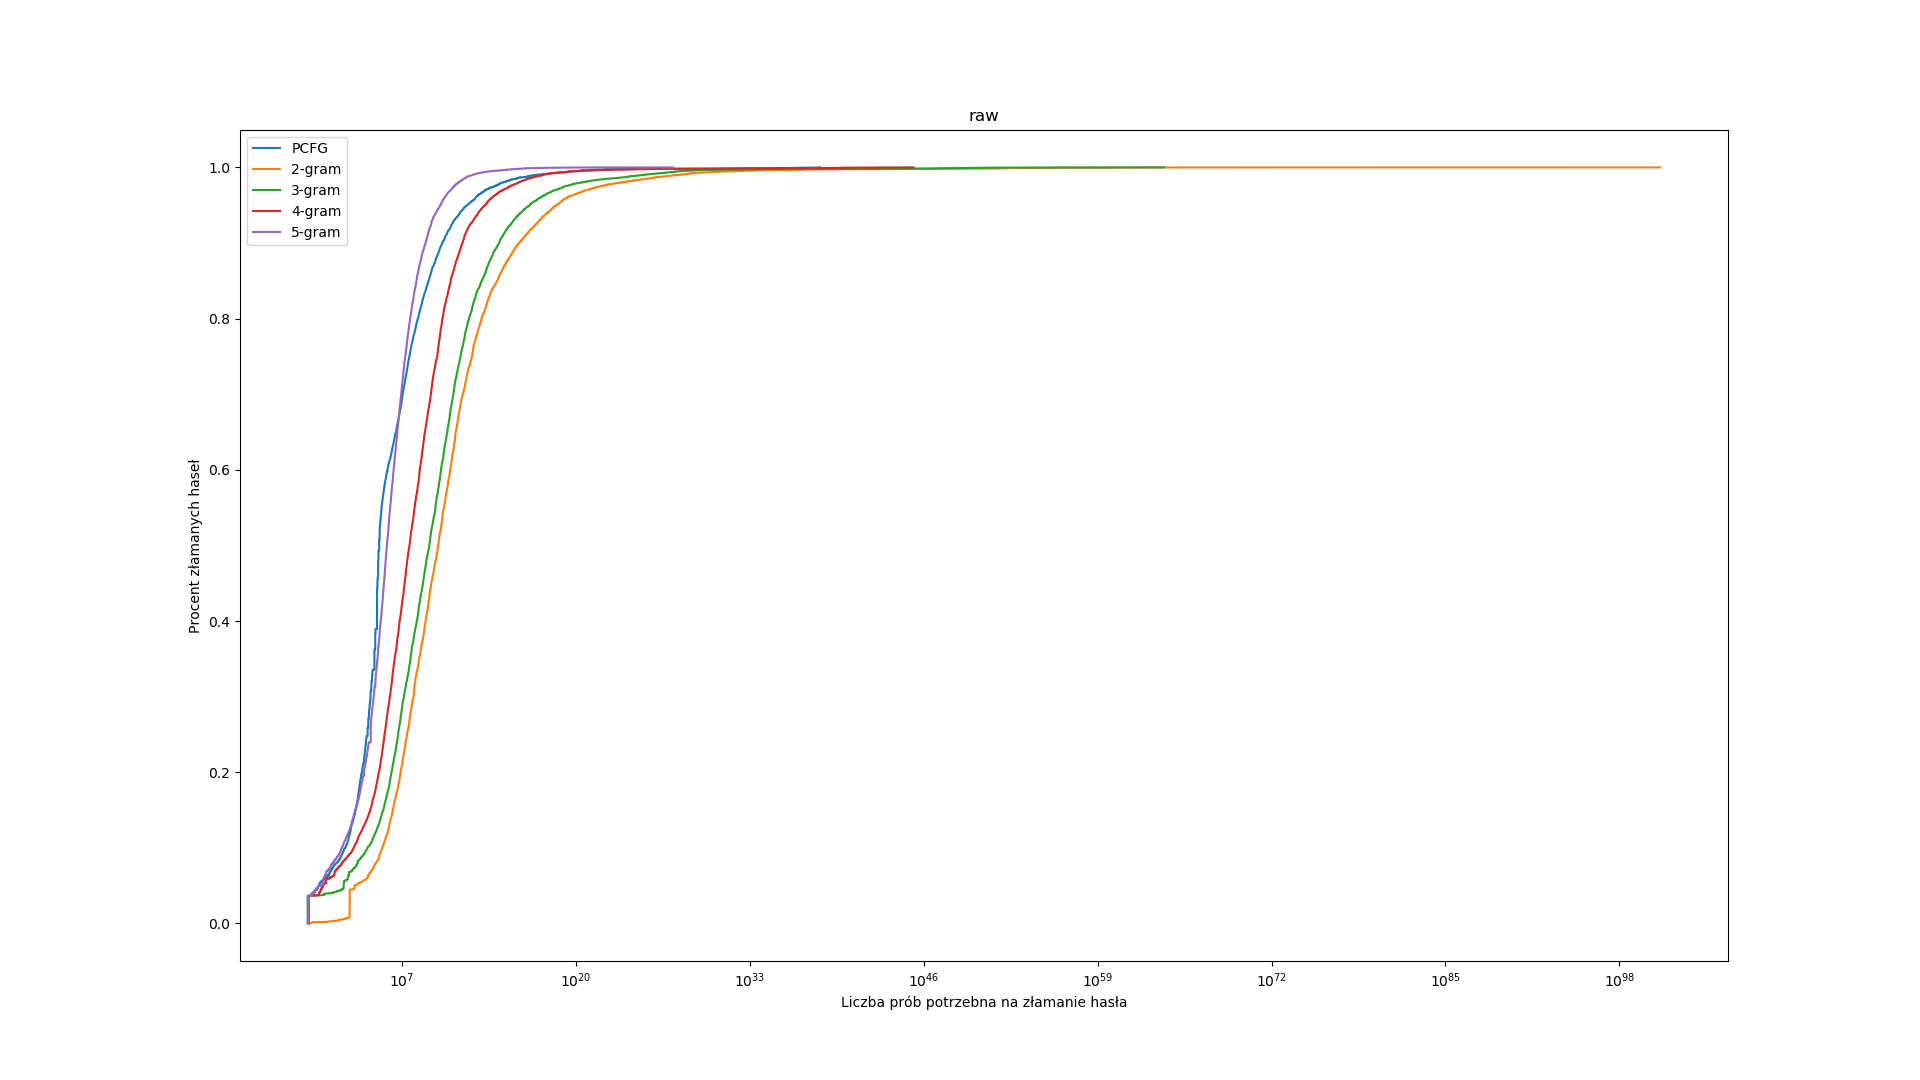
\includegraphics{raw}
		\caption{Wpływ rodzaju algorytmu na liczbę prób potrzebnych do złamania haseł nienależących do żadnej polityki}
	\end{figure}

	\begin{figure}[H]
		\centering
		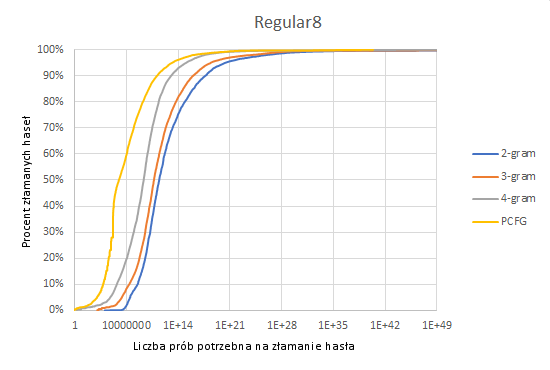
\includegraphics{regular8}
		\caption{Wpływ rodzaju algorytmu na liczbę prób potrzebnych do złamania haseł w polityce regular8}
	\end{figure}

	\begin{figure}[H]
		\centering
		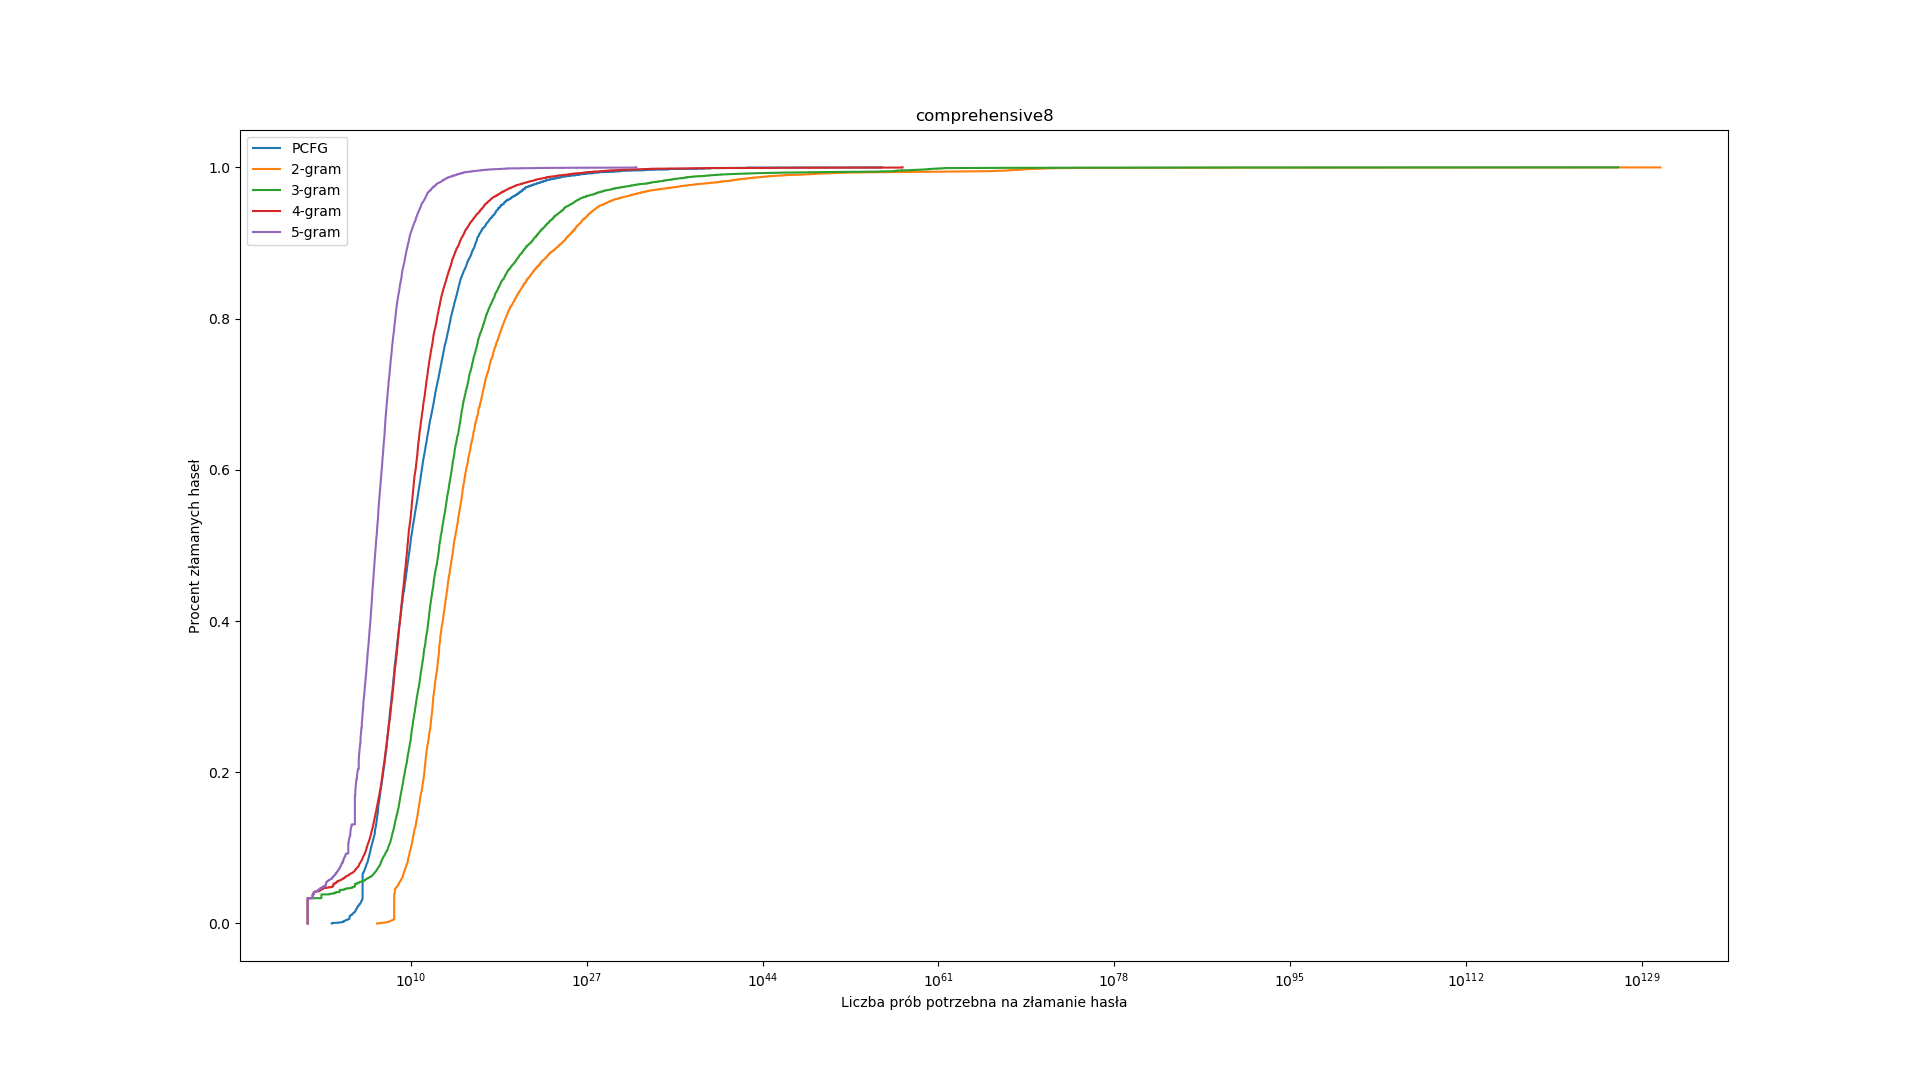
\includegraphics{comprehensive8}
		\caption{Wpływ rodzaju algorytmu na liczbę prób potrzebnych do złamania haseł w polityce comprehensive8}
	\end{figure}


	Rysunki 1, 2 i 3 przedstawiają ile faktycznych prób musi wykonać każdy z algorytmów, aby odgadnąć procentową część wszystkich haseł z ciągu walidacyjnego.

	\subsection{Porównanie wpływu rodzaju algorytmu na skuteczność łamania haseł w każdej z polityk}
	\begin{figure}[H]
		\centering
		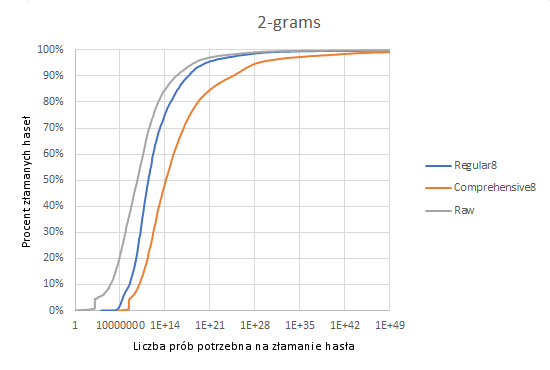
\includegraphics{2grams}
		\caption{Skuteczność łamania haseł dla każdej polityki w algorytmie bazującym na 2-gramach (standardowy BFM)}
	\end{figure}

	\begin{figure}[H]
		\centering
		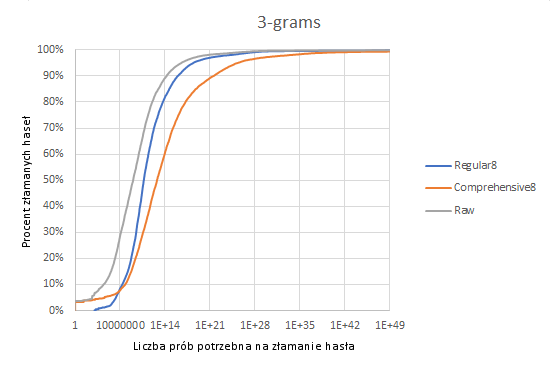
\includegraphics{3grams}
		\caption{Skuteczność łamania haseł dla każdej polityki w algorytmie bazującym na 3-gramach}
	\end{figure}

	\begin{figure}[H]
		\centering
		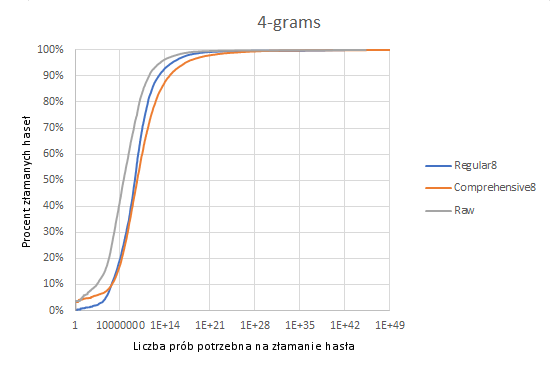
\includegraphics{4grams}
		\caption{Skuteczność łamania haseł dla każdej polityki w algorytmie bazującym na 4-gramach}
	\end{figure}

	\begin{figure}[H]
		\centering
		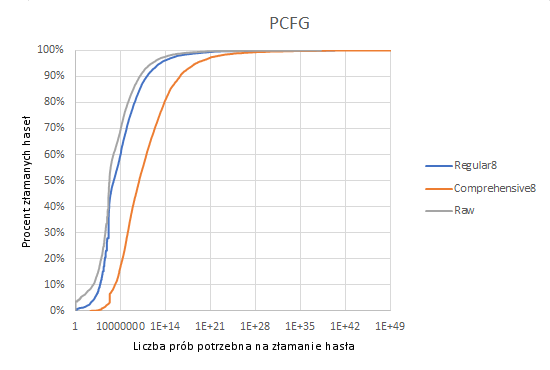
\includegraphics{PCFG}
		\caption{Skuteczność łamania haseł dla każdej polityki w algorytmie PCFG (algorytmie Weira)}
	\end{figure}

	Rysunki 4, 5, 6 i 7 przedstawiają liczbę prób potrzebną do złamania procentowej części wszystkich haseł z ciągu walidacyjnego.

	%----------------------------------------------------------------------------------------
	%	SECTION 5
	%----------------------------------------------------------------------------------------
	\newpage
	\section{Analiza wyników}
	\subsection{Analiza wpływu polityki tworzenia haseł i rodzaju używanego algorytmu na skuteczność łamania haseł}
		Przeprowadzone badania potwierdzają zależność pomiędzy stopniem złożoności algorytmu a jego skutecznością
		niezależnie od wybranej polityki tworzenia haseł. Algorytm PCFG, który przeprowadza najbardziej szczegółową
		analizę haseł z ciągu treningowego, wyprzedza wszystkie algorytmy bazujące na n-gramach w liczbie prób, potrzebnych
		do złamania hasła. Podczas porównywania ze sobą n-gramów, również obserwowany jest wpływ długości ciągów znaków
		na skuteczność algorytmu - niezależnie od rodzaju łamanych haseł dłuższy ciąg znaków skutkował większą efektywnością.

		W oparciu o rysunek 3 przy polityce comprehensive8 można zauważyć przewagę w skuteczności algorytmu
		opierającego się na 4-gramach nad algorytmem PCFG w ponad \textit{50\%} badanych haseł z ciągu walidacyjnego.
		Aby potwierdzić zależność pomiędzy tą konkretną polityką a skutecznością obu algorytmów, warto wykonać powtórne
		testy na większym zbiorze treningowym.

		Zarówno w przypadku algorytmów opierających się o 2-gramy, jak i 3-gramy, widoczna jest różnica wpływu polityki
		tworzenia haseł na ich siłę (w kontekście ich łamania przez w. w. algorytmy). Hasła, które nie miały żadnych
		zasad regulujących strukturę ich tworzenia, były bardziej podatne na złamanie niż w przypadku polityki regular8
		czy comprehensive8. Wśród tych dwóch polityk z kolei w około \textit{90\%} przypadków silniejsze były hasła,
		których struktura zawierała minimum jeden znak specjalny, jedną cyfrę i jedną wielką literę.

		W przypadku algortmów opierających się na 4-gramach różnice w sile haseł w zależności od polityki są o wiele mniejsze
		niż w przypadku 2-gramów czy 3-gramów. Wciąż można zaobserwować taką samą tendencję, jednak w szczególności
		polityki regular8 i comprehensive8 zbliżają się do siebie swoją podatnością na złamanie.

		W przypadku algorytmu PCFG różnice w sile haseł są nieco większe - widoczna jest duża przewaga haseł w polityce
		comprehensive8 nad innymi politykami. Zacierają się jednak różnice w podatności na łamanie haseł z kategorii raw
		i regular8.

	%----------------------------------------------------------------------------------------
	%	SECTION 6
	%----------------------------------------------------------------------------------------
	%\newpage
	\section{Podsumowanie}
	
	%----------------------------------------------------------------------------------------
	\newpage
	\bibliography{bibliography}
	
\end{document}